经典的电动力学 (或经典电磁学) 研究的是 (真空中的) {\bf 麦克斯韦方程}
\begin{align*}
    \nabla\cdot E&=\frac{\rho}{\varepsilon_0}, \tag{高斯定理}\\
    \nabla\cdot B&= 0, \tag{高斯磁定律}\\ 
    \nabla\times E&=-\frac{\partial B}{\partial t}, \tag{法拉第电磁感应定律}\\
    \nabla\times B&=\mu_0 J+\mu_0\varepsilon_0\frac{\partial E}{\partial t}. \tag{麦克斯韦-安培定律}
\end{align*}
其中 $ E $ 是电场, $ B $ 是磁场, $ \rho $ 是电荷密度, $ \varepsilon_0\approx 8.854187817\times 10^{-12}\text{A}^2\cdot\text{s}^4\cdot\text{kg}^{-1}\cdot\text{m}^{-3} $ 是真空电容率, $ \mu_0\approx 1.2566370614\times 10^{-6} \text{N}\cdot\text{A}^{-2} $ 是真空磁导率, $ J $ 是电流密度.

其中高斯定律描述了电荷如何产生电场, 高斯磁定律指出磁场是无源场 (即不存在磁单极子), 法拉第电磁感应定律描述了磁生电, 麦克斯韦-安培定律描述了电生磁.

若不存在源电流 ($J=0$) 与源电荷 ($\rho=0$), 则麦克斯韦方程组为
\begin{align*}
    \nabla\cdot E&=0,\\
    \nabla\cdot B&=0,\\ 
    \nabla\times E&=-\frac{\partial B}{\partial t},\\
    \nabla\times B&=\mu_0\varepsilon_0\frac{\partial E}{\partial t}.
\end{align*}
对后两个式子取旋度, 可得
\begin{align*}
    \nabla\times(\nabla\times E) &= -\frac{\partial}{\partial t}(\nabla\times B)=-\mu_0\varepsilon_0\frac{\partial^2 E}{\partial t^2},\\ 
    \nabla\times(\nabla\times B) &= \mu_0\varepsilon_0\frac{\partial}{\partial t}(\nabla\times E)=-\mu_0\varepsilon_0\frac{\partial^2 B}{\partial t^2}.
\end{align*}
应用恒等式
\[ \nabla\times(\nabla\times A)=\nabla(\nabla\cdot A)-\nabla^2 A \]
可进一步得到
\[ \begin{aligned}
    \left( \nabla^2-\mu_0\varepsilon_0\frac{\partial^2}{\partial t^2} \right)E &=0,\\ 
    \left( \nabla^2-\mu_0\varepsilon_0\frac{\partial^2}{\partial t^2} \right)B &=0.
\end{aligned} \]
这个方程叫做{\bf 亥姆霍兹方程} (Helmholtz equation), 将其与波动方程
\[ \frac{\partial^2 u}{\partial t^2}=c^2\nabla^2 u \]
(其中 $ c $ 代表波的传播速率) 进行对照可知此时的电和磁形如传播速率为
\[ c=\frac{1}{\sqrt{\mu_0\varepsilon_0}}\approx 299\ 792\ 458 \text{ m/s} \] 
的波 (电磁波). 但这也导致了一个``问题'': 由于麦克斯韦方程组在所有惯性坐标系中的形式都是一样的, 因此通过上述方式推导出的电磁波的传播速率在所有惯性系中也都相同, 这与人们经典物理学中对速度的认知相违背, 这一矛盾后来催生出了狭义相对论.

因此, 本章主要介绍狭义相对论. 
\begin{remark}
本章所涉及的数学前置知识见附录 \ref{differential geometry}, 其中有几点需要特殊强调:
\begin{enumerate}
    \item 度量可以不是正定的 (定义 \ref{metric});
    \item 记号说明见附录 \S\, \ref{notation}.
\end{enumerate}
\end{remark}

\section{相对论基础概念}
狭义相对论的基本假设有两条:
\begin{enumerate}
    \item {\bf 光速不变原理}: 在所有惯性系中真空光速都为 $ c $ (今后若无特殊声明, 均采用几何单位制 $ c=1 $).
    \item {\bf 狭义相对性原理}: 所有惯性系平权, 即所有惯性系中物理定律的表达形式相同.
\end{enumerate}
\subsection{时空}
很自然地, 我们可以认为每一事件都发生在空间的一点 $ x $ 和时间的一瞬 $ t $, 于是我们也反过来称 $ (x,t) $ 为一个{\bf 事件} (event). 全部事件构成的集合叫做{\bf 时空} (spacetime), 一般我们假定时空是一个 $ 4 $ 维流形.

有线性代数的知识, 对于任意有限维线性空间 $ V $ 上的任意度量 $ g $, 必存在一组正交归一基, 使得 $ g $ 在这组基上的表示为对角阵, 且对角元的正负个数 (正负惯性指数) 与基的选取无关. 我们称正惯性指数减去负惯性指数所得结果为{\bf 号差} (signature).

用正交归一基将度量表示为对角矩阵后, 称对角元全为 $ +1 $ 的度量为{\bf 正定度量}或{\bf 黎曼度量} (Riemannian metric), 称恰好有一个对角元为 $ -1 $, 其余对角元均为 $ +1 $ 的度量为{\bf 洛伦兹度量} (Lorentzian metric).

\begin{remark}
    也有资料将洛伦兹度量定义为只有一个对角元为 $ +1 $, 其余对角元均为 $-1$ 的度量, 在本书的量子场论章节, 将会采用这种定义.
\end{remark}

\begin{enumerate}
    \item 经典物理假定时空流形为 $ \mathbb{R}^4 $, 其上配有正定度量. 设 $ \{x^\alpha\} $ 为 $ \mathbb{R}^n $ 的坐标, 则张量场 $ \delta:=\delta_{\alpha\beta}\,\mathrm{d}x^\alpha\otimes\mathrm{d}x^\beta $ 叫做{\bf 欧氏度量}, 二元组 $ (\mathbb{R}^n,\delta) $ 叫做{\bf 欧式空间}或{\bf 欧式时空}, 其中
    \[ \delta_{\alpha\beta}=\begin{cases}
        0, & \alpha\neq\beta,\\ +1, & \alpha=\beta.
    \end{cases} \]
    \item 狭义相对论也假定时空流形为 $ \mathbb{R}^4 $, 但其上配有洛伦兹度量. 设 $ \{x^\alpha\} $ 为 $ \mathbb{R}^n $ 的坐标, 则张量场 $ \eta:=\eta_{\alpha\beta}\,\mathrm{d}x^\alpha\otimes\mathrm{d}x^\beta $ 叫做{\bf 闵氏度量} (Minkowski metric), 二元组 $ (\mathbb{R}^n,\eta) $ 叫做{\bf 闵式空间}或{\bf 闵氏时空}, 其中
    \[ \eta_{\alpha\beta}=\begin{cases}
        0, & \alpha\neq\beta,\\ -1, & \alpha=\beta=0,\\ +1, & \alpha=\beta=1,\dots,n-1.
    \end{cases} \]
    \item 广义相对论允许时空流形为任意 $ 4 $ 维连通流形, 其上配有洛伦兹度量. 这样的流形叫做{\bf 伪黎曼流形}或{\bf 伪黎曼时空}.
\end{enumerate}

狭义相对论研究的就是 $ 4 $ 维闵氏时空的几何. 由 $\eta_{\alpha\beta}$ 的值来看, 第一个坐标分量是特殊的. 实际上, 我们总是用第一个坐标分量来表示时间, 因此, 我们对于张量的指标做以下约定:
\begin{itemize}
    \item 用希腊字母 $\alpha,\beta,\mu,\nu,\dots$ 来表示可以取 $0,1,2,3$ 的指标;
    \item 用从 $ i $ 开始的字母 $ i,j,k,\dots $ 来表示只能取 $1,2,3$ 的指标.
\end{itemize}

给定坐标系 $\{x^\alpha\}$, 借由 $\eta$ 来升降指标, 容易验证
\begin{align*}
    v^0 &=v(\mathrm{d}x^0)=v^\alpha(\mathrm{d}x^0)_{\alpha}\\
    &=\eta^{\alpha\beta}v_{\beta}(\mathrm{d}x^0)_{\alpha}=\eta^{00}v_{0}(\mathrm{d}x^0)_{0}=-v_0.
\end{align*}
类似地有 $v^i=v_i$ (其他类型张量的情况也类似). 因此, 指标 $0$ 的升降会导致一个负号, 而指标 $1,2,3$ 的升降不改变系数的值.

\subsection{光速不变原理}
\label{line element}
\begin{definition}
    给定线性空间 $ V $ 上的洛伦兹度量 $ g $, 我们将 $ V $ 中的向量分为三类:
    \begin{enumerate}
        \item 满足 $ g(v,v)<0 $ 的 $ v $ 叫做{\bf 类时向量} (timelike vector);
        \item 满足 $ g(v,v)=0 $ 的 $ v $ 叫做{\bf 类光向量} (lightlike vector);
        \item 满足 $ g(v,v)>0 $ 的 $ v $ 叫做{\bf 类空向量} (spacelike vector).
    \end{enumerate}
\end{definition}

\begin{definition}[曲线长度]
    对于配有洛伦兹度量 $ g $ 的流形 $ M $, 若其上的 $ C^1 $ 曲线 $ C(t) $ 的每一点的切向量都类时, 则称其为类时曲线, 类似地可以定义类光曲线和类空曲线. 进一步地, 定义这三种曲线从 $ t_1 $ 到 $ t_2 $ 的{\bf 长度}为
    \[ l:=\int_{t_1}^{t_2}\sqrt{|g(T,T)|}\,\mathrm{d}t,\quad T=\frac{\mathrm{d} C(t)}{\mathrm{d} t}. \]
\end{definition}

\begin{remark}
    我们只对这三种曲线定义了长度, 且类光曲线的长度恒为 $ 0 $.
\end{remark}
设曲线 $C(t)$ 在坐标系 $\{x^\alpha\}$ 下的参数表达为 $(x^\alpha(t))$, 则
\[ g(T,T)=g\left( T^\alpha\frac{\partial}{\partial x^\alpha},T^\beta\frac{\partial}{\partial x^\beta} \right)=T^\alpha T^\beta g\left( \frac{\partial}{\partial x^\alpha},\frac{\partial}{\partial x^\beta} \right)=\frac{\mathrm{d}x^\alpha}{\mathrm{d}t}\frac{\mathrm{d}x^\beta}{\mathrm{d}t}g_{\alpha\beta}, \]
因此曲线长度可表达为
\[ l=\int_{t_1}^{t_2}\sqrt{g_{\alpha\beta}\frac{\mathrm{d} x^\alpha}{\mathrm{d} t}\frac{\mathrm{d} x^\beta}{\mathrm{d} t}}\,\mathrm{d} t. \] 
为了方便书写我们还可以引入{\bf 线元} (line element) 记号 
\[ \mathrm{d}s^2:=g_{\alpha\beta}\,\mathrm{d}x^\alpha\mathrm{d}x^\beta. \] 
\begin{remark}
    这里我们记 $\mathrm{d}x^{\alpha}\mathrm{d}x^{\beta}:=\mathrm{d}x^{\alpha}\otimes\mathrm{d}x^{\beta}$, 因此线元只是度量的另一种写法. 
\end{remark}

在洛伦兹坐标系下, 线元为
\[ \mathrm{d}s^2=-(\mathrm{d}x^0)^2+(\mathrm{d}x^1)^2+(\mathrm{d}x^2)^2+(\mathrm{d}x^3)^2. \]
由于我们用第一个坐标分量 $ x^0 $ 来表示时间, 因此也将坐标系 $ \{x^0,x^1,x^2,x^3\} $ 写作 $ \{t,x,y,z\} $, 此时线元为
\[ \mathrm{d}s^2=-\mathrm{d}t^2+\mathrm{d}x^2+\mathrm{d}y^2+\mathrm{d}z^2. \]

质点是牛顿力学中的概念, 指的是空间中带有质量的点, 这里我们将其推广为{\bf 粒子} (particle) 概念, 粒子分为两种: 
\begin{enumerate}
    \item 有 (静) 质量的粒子, 也叫作{\bf 质点}.
    \item 无 (静) 质量的粒子, 也叫做{\bf 光子}(photon).
\end{enumerate}
一个粒子的全部历史由一系列事件组成, 对应时空中的一条曲线, 该曲线叫做该粒子的{\bf 世界线} (world line). 

给定一个粒子的世界线 $ (t,x(t),y(t),z(t)) $, 我们熟知的速率可定义为
\[ v:=\frac{\sqrt{\mathrm{d}x^2+\mathrm{d}y^2+\mathrm{d}z^2}}{\mathrm{d}t}, \]
上式可改写为
\[ \mathrm{d}s^2=-(1-v^2)\,\mathrm{d}t^2. \]
这说明狭义相对论中的两个假设
\begin{enumerate}
    \item (光速不变原理) 光子相对于任意惯性系的速率为 $ 1 $.
    \item 质点相对于任意惯性系的速率小于光速 $ 1 $.
\end{enumerate}
可被重新表述为下面两个公理 (暂时忽略惯性系概念):
\begin{enumerate}
    \item 光子世界线为类光曲线 ($ \mathrm{d}s^2=0 $).
    \item 质点世界线为类时曲线 ($ \mathrm{d}s^2<0 $).
\end{enumerate}

\subsection{狭义相对性原理}
我们将进行物理观测的人视为质点, 称其为{\bf 观者} (observer), 观者手中有一个{\bf 标准钟} (standard clock), 该钟的读数叫做该观者的{\bf 固有时} (proper time), 一个观者的固有时是该观者自身所经历的时间. 而每点的第一个坐标分量叫做该坐标系下的{\bf 坐标时} (coordinate time).

\begin{remark}
    严谨地说, 观者是配有正交归一标架场的类时曲线.
\end{remark}

\begin{definition}[标准钟]
    若一个钟在自己世界线上任意两点 $ p_1,p_2 $ 的读数 $ \tau_1,\tau_2 $ 之差为 $ p_1,p_2 $ 之间的线长, 则我们称它为{\bf 标准钟}或{\bf 理想钟} (ideal clock).
\end{definition}

\begin{remark}
    今后谈及世界线时默认以固有时 $ \tau $ 为参数, 由于固有时等于线长, 其切向量的长度为 $ 1 $. 
\end{remark}

推而广之, 我们可以认为每个质点都是一个观者, 有自己的固有时. 但光子没有固有时, 不能充当观者.

如果一个由观者构成的集合 $ \mathcal{R} $ 满足时空 (或其中任意开子集) 中每一点恰有 $ \mathcal{R} $ 内的一个观者的世界线经过, 则称 $ \mathcal{R} $ 为一个 (局部) {\bf 参考系} (reference frame). 

想象每个观者带有一个标准钟, 其读数为 $ t $, 且身上标有三个实数 $ (x,y,z) $, 则任一事件必发生在某一观者身上, 它可以记录下该事件的时空坐标 $ \{t,x,y,z\} $. 有时我们也反过来用坐标 $\{t,x,y,z\}$ 来代指相应的参考系.

狭义相对性原理指出存在一类特殊的观者是惯性 (inertial) 观者, 且它们相互之间平权, 不存在特殊的惯性观者, 比如不能说哪个惯性观者是绝对静止的. 一族惯性观者构成的参考系叫做惯性参考系.

若一个质点的世界线为测地线 (定义 \ref{geodesic}), 则称该质点为``自由的''或``做惯性运动的'', 其对应的观者叫做{\bf 惯性观者}. 由惯性观者构成的参考系叫做{\bf 惯性参考系}, 属于同一惯性参考系的所有观者的世界线是相互平行的测地线. 以观者的固有时作为 $ t $ 坐标所得到的坐标系叫做{\bf 惯性坐标系}. 在不需要区分参考系和坐标系时, 我们将惯性参考系和惯性坐标系统称为{\bf 惯性系}. 
\begin{remark}
    严谨地说, 惯性观者是做惯性运动的无自转观者 (详见 \S\,\ref{rotation}). 在狭义相对论中, 与惯性系坐标 $\{t,x,y,z\}$ 对应的标架
    \[ \left\{\frac{\partial}{\partial t},\,\frac{\partial}{\partial x},\,\frac{\partial}{\partial y},\,\frac{\partial}{\partial z}\right\}, \]
    能保证观者是无自转的, 因此不用担心这个问题.
\end{remark}
定义{\bf 洛伦兹系}为闵氏时空中满足
\[ \eta\left( \frac{\partial}{\partial x^\alpha},\frac{\partial}{\partial x^\beta} \right)=\eta_{\alpha\beta} \]
的坐标系 $ \{x^0,x^1,x^2,x^3\} $. 于是洛伦兹系之间的变换对应于 $ (\mathbb{R}^4,\eta) $ 中的等距微分同胚 \cite[定理 4-3-6]{梁灿彬2000微分几何入门与广义相对论}, 而任一等距微分同胚可由以下几类基本的等距微分同胚复合而成 \cite[上册 136 页]{梁灿彬2000微分几何入门与广义相对论}:
\begin{enumerate}
    \item 空间反射, 如 $ x'= -x $.
    \item 时间反演 $ t'=-t $.
    \item 平移, 如 $ t'=t+a $ 和 $ x'=x+a $.
    \item 空间旋转, 如 $\ \begin{aligned}
            x'&=x\cos\theta-y\sin\theta,\\
            y'&=x\sin\theta+y\cos\theta.
    \end{aligned}$
    \item {\bf 洛伦兹变换}, 如 $\ \begin{aligned}
        t'&=t\cosh\alpha-x\sinh\alpha,\\
        x'&=-t\sinh\alpha+x\cosh\alpha.
    \end{aligned}$.
\end{enumerate}

第一类变换会改变手性, 第二类变换会改变时间方向, 它们都是在重新设定坐标轴方向, 我们不关心这些变换, 以后不再讨论它们. 后三类变换是我们所关心的, 实际上, 后三类变换所生成的洛伦兹系 (即保持时间方向和手性的等距微分同胚所对应的坐标系) 恰是惯性系; 反之, 惯性系也都是这样的洛伦兹系.
\begin{remark}
    因此惯性系可以视作所有坐标系商掉一个等价关系后的一个等价类, 这是狭义相对性原理的数学体现. 注意 $\mathbb{R}^4$ 自然拥有的坐标系显然是惯性系, 因此我们已经先钦定了一个惯性系等价类的代表元.
\end{remark}
接下来讨论后三类变换. 平移是在重新设置初始值 (原点), 空间旋转是在重新设置 $x,y,z$ 轴的方向. 对于洛伦兹变换, 我们也将其写作 
\begin{align*}
    t' &= \gamma\left(t-\frac{vx}{c^2}\right),\\ 
    x' &= \gamma(x-vt),
\end{align*}
其中
\[ \gamma:=\frac{1}{\sqrt{1-\frac{v^2}{c^2}}} \] 
叫做{\bf 洛伦兹因子}. 这对应于两个惯性系 $ \mathcal{R}' $ 和 $ \mathcal{R} $ 之间的坐标变换, 两个坐标系的坐标轴分别平行且朝向相同, $ \mathcal{R}' $ 相对与 $ \mathcal{R} $ 以速率 $ v $ 沿 $ x $ 轴正向匀速移动. 若定义{\bf 快度}(rapidity)为 
\[ \alpha=\mathrm{arctanh}\left( \frac{v}{c} \right),\] 
则 $\gamma=\cosh\alpha$ 且洛伦兹变换可写为
\[ \left(\begin{matrix}
   ct' \\ x' 
\end{matrix}\right)=\left(\begin{matrix}
    \cosh\alpha & -\sinh\alpha\\ 
    -\sinh\alpha & \cosh\alpha
\end{matrix}\right)\left(\begin{matrix}
    ct \\ x
\end{matrix}\right), \]
这就是前文给出的双曲函数形式的洛伦兹变换, 其逆变换为
\[ \left(\begin{matrix}
    ct \\ x
\end{matrix}\right)=\left(\begin{matrix}
    \cosh\alpha & \sinh\alpha\\ 
    \sinh\alpha & \cosh\alpha
\end{matrix}\right)\left(\begin{matrix}
    ct' \\ x'
\end{matrix}\right). \]

\begin{figure}[H]
    \centering
    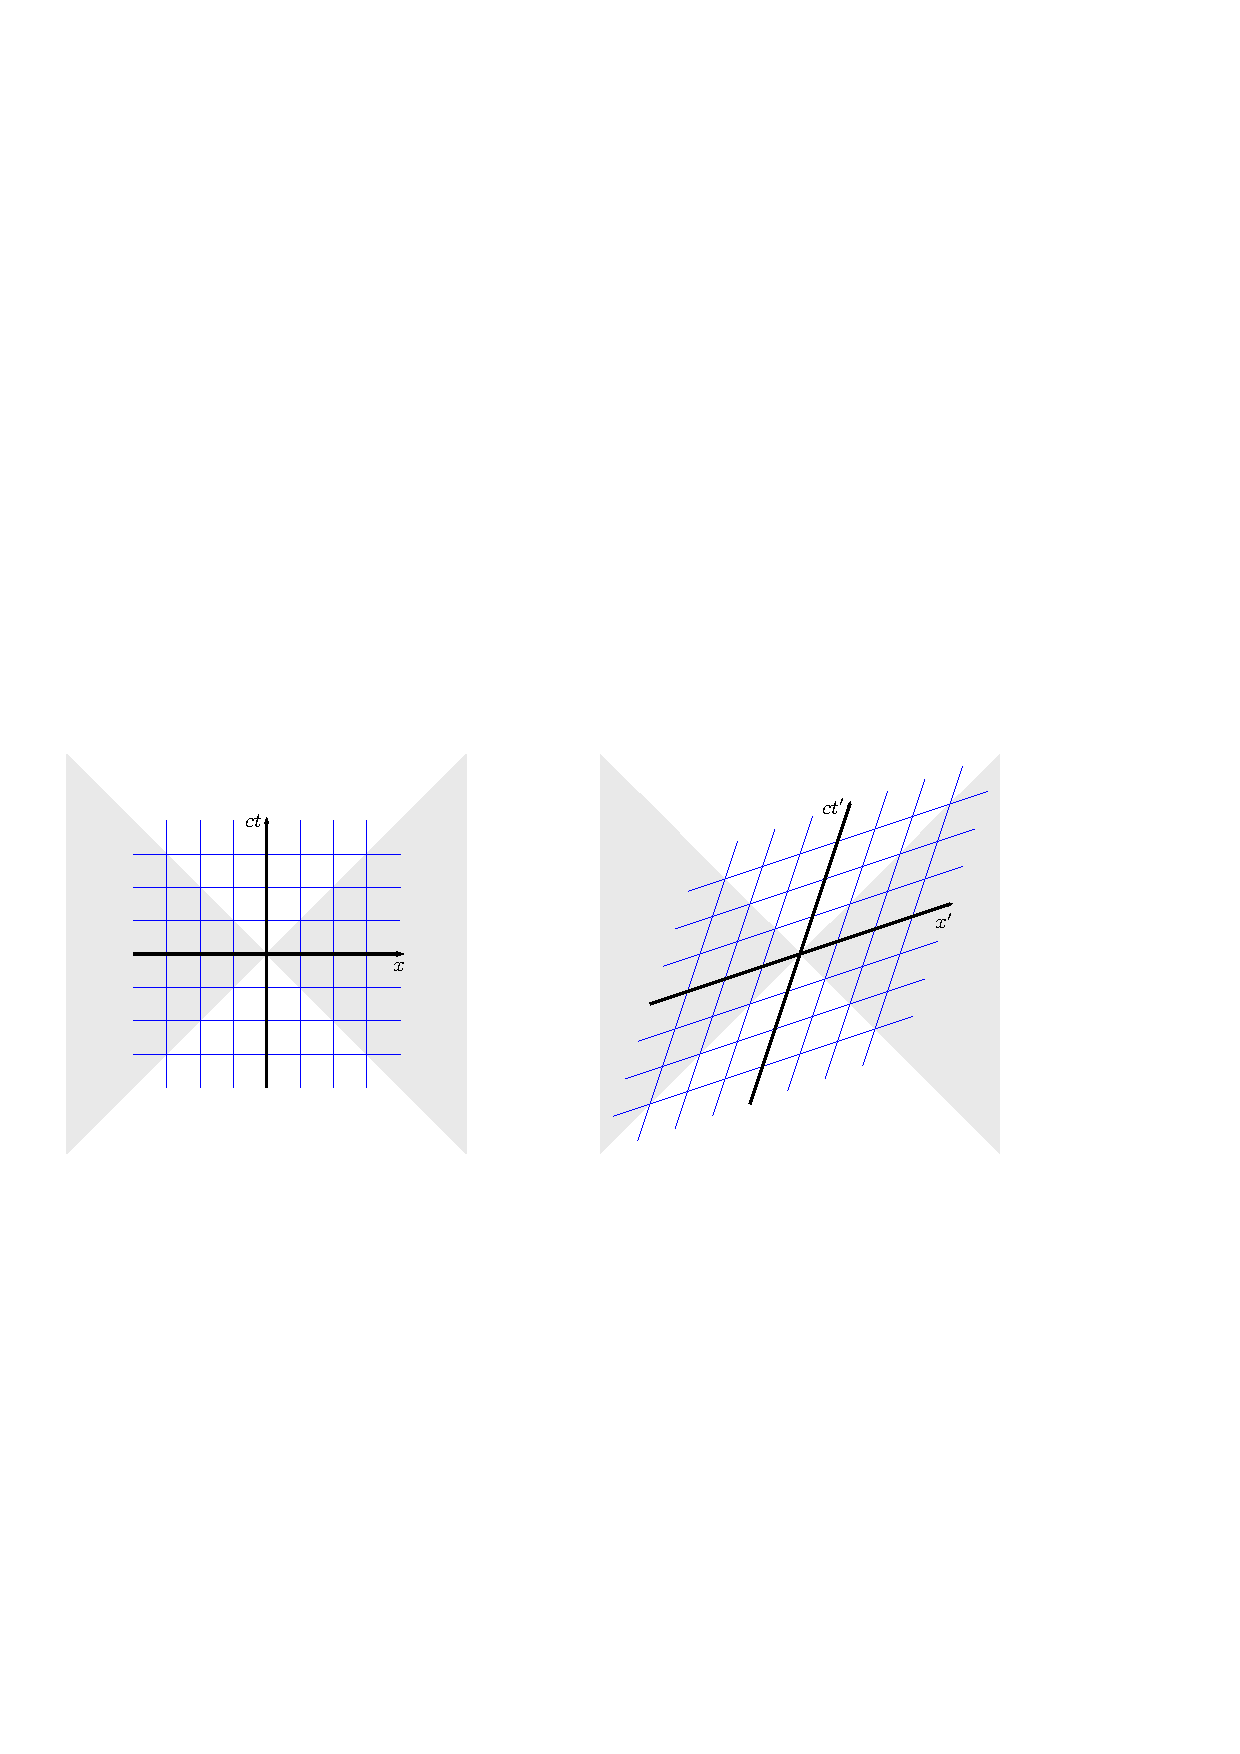
\includegraphics[width=0.85\textwidth]{pic/Lorentz transform.pdf}
    \caption{Lorentz transform}
    \label{Lorentz transform}
\end{figure}

以牛顿力学的角度来看, 不能超光速略显奇怪; 如今在狭义相对论中, 速度不能叠加, 但由    
\[ \left(\begin{matrix}
    \cosh\alpha_1 & \sinh\alpha_1\\ 
    \sinh\alpha_1 & \cosh\alpha_1
\end{matrix}\right)\left(\begin{matrix}
    \cosh\alpha_2 & \sinh\alpha_2\\ 
    \sinh\alpha_2 & \cosh\alpha_2
\end{matrix}\right)=\left(\begin{matrix}
    \cosh(\alpha_1+\alpha_2) & \sinh(\alpha_1+\alpha_2)\\ 
    \sinh(\alpha_1+\alpha_2) & \cosh(\alpha_1+\alpha_2)
\end{matrix}\right) \] 
知同一方向上的快度是可以叠加的, 若利用快度来进行思考, 由 $\mathrm{arctanh}$ 的图像知光速对应着 $\infty$ 快度, 这显然不能被超越的, 甚至是无法达到的.